\section{Project Plan}

\subsection{Aim of the Project}

The overarching goal of this research is to address the pervasive issue of temporal awareness in Large Language Model (LLM)-based information retrieval systems, specifically within the context of ChatUQ, a chatbot under development for the University of Queensland. The lack of temporal awareness in such systems manifests as a deficiency in processing and responding accurately to time-sensitive queries, crucial for effective user interaction. This project aims to systematically quantify the problem of temporal awareness, identify potential solutions from existing literature, and develop novel methodologies that can be integrated into the retrieval-augmented generation (RAG) framework of ChatUQ. Key objectives include: \\

\begin{itemize}
    \item Quantifying Temporal Awareness Deficiencies: Determine the frequency and conditions under which temporal misunderstandings occur within LLMs.
    \item Development and Refinement of a Dataset: Create and utilize a dataset consisting of diverse temporal queries to measure and enhance the temporal accuracy of response generation in LLM-based IR systems.
    \item Exploration and Adaptation of Existing Solutions: Investigate current methodologies addressing similar issues in other contexts and adapt these solutions.
    \item Tailoring of New Methodologies: Develop and test new approaches that explicitly address shortcomings of existing solutions.
    \item Evaluation and Future Planning: Assess the effectiveness of implemented solutions and establish a road map for ongoing enhancement and integration.
\end{itemize}

By achieving these aims, the project will significantly advance the temporal processing capabilities of ChatUQ, setting a benchmark for LLM-based systems in handling time-critical information requests.

\subsection{Methodology}

\subsubsection{Measuring Temporal Comprehension}

\begin{itemize}
    \item Incidence Tracking: Establish a systematic approach to track and analyze incidents of temporal misunderstandings within LLM interactions.
    \item Experimental Validation: Conduct controlled experiments to validate the findings from the incidence tracking.
\end{itemize}

\subsubsection{Dataset Creation}

\begin{itemize}
    \item Query Generation: Utilize both manual creation and LLM-generated prompts to compile a comprehensive dataset of temporal queries relevant to the university context, such as event dates and historical data inquiries.
    \item Evaluation Criteria Establishment: Implement human annotation to determine the presence of temporal comprehension issues within responses. Deciding what evaluation tools could be used such as precision, Z-Tests for Proportions or binomial tests to validate the significance of findings based on the dataset's diversity and size.
\end{itemize}



\subsubsection{Literature Review}

\begin{itemize}
    \item Source Identification: Conduct a thorough search on databases like Google Scholar using keywords related to temporal awareness in LLMs and RAG systems, focusing on fields like Natural Language Processing and Information Retrieval.
    \item Paper Categorization: Manually categorize identified papers based on their methodology's relevance and applicability to the project's goals. Methods will be classified as directly applicable, adaptable, inspirational, or not useful, depending on their potential to address the specific needs of ChatUQ.
    \item Analyze the Papers: Identify baselines that could be implemented and existing methods that could be adapted. Further, report shortcomings of current methods.
\end{itemize}

\subsubsection{Refining Methodologies}

\begin{itemize}
    \item Improvement and Adaptation: Based on insights gained from the literature review, improve on existing methods by creating new methods or adapt existing ones to improve temporal accuracy in ChatUQ. This phase focuses on integrating effective strategies into the RAG framework, considering computational and data constraints.
    \item Prototyping: Implement these methods within a controlled environment to test their initial effectiveness and integration with existing systems.
\end{itemize}

\subsubsection{Evaluation}

\begin{itemize}
    \item Performance Analysis: Compare and contrast the enhanced system using the specially created dataset with the existing system to evaluate improvements in temporal awareness.
    \item Gap Identification and Planning: Identify any remaining gaps in temporal comprehension and outline future research directions and enhancements. This includes planning for scalability and deeper integration of successful methodologies.
\end{itemize}

This comprehensive methodology aims not only to enhance ChatUQ's functionality but also to contribute to the broader academic and practical applications of LLM technologies, particularly in their ability to interact more naturally and effectively with human users in time-sensitive contexts.

\subsection{Milestones and Timeline}

% \begin{center}
% \begin{tabular}{|c|c|c|}
% \hline
% \textbf{Semester No./Week No.} & \textbf{Milestones} & \textbf{Description} \\
% \hline
% S1/W5 & Writing Task & Submit the final Writing Task on Blackboard \\
% \hline
% Row2Cell1 & Row2Cell2 & Row2Cell3 \\
% \hline
% \end{tabular}
% \end{center}

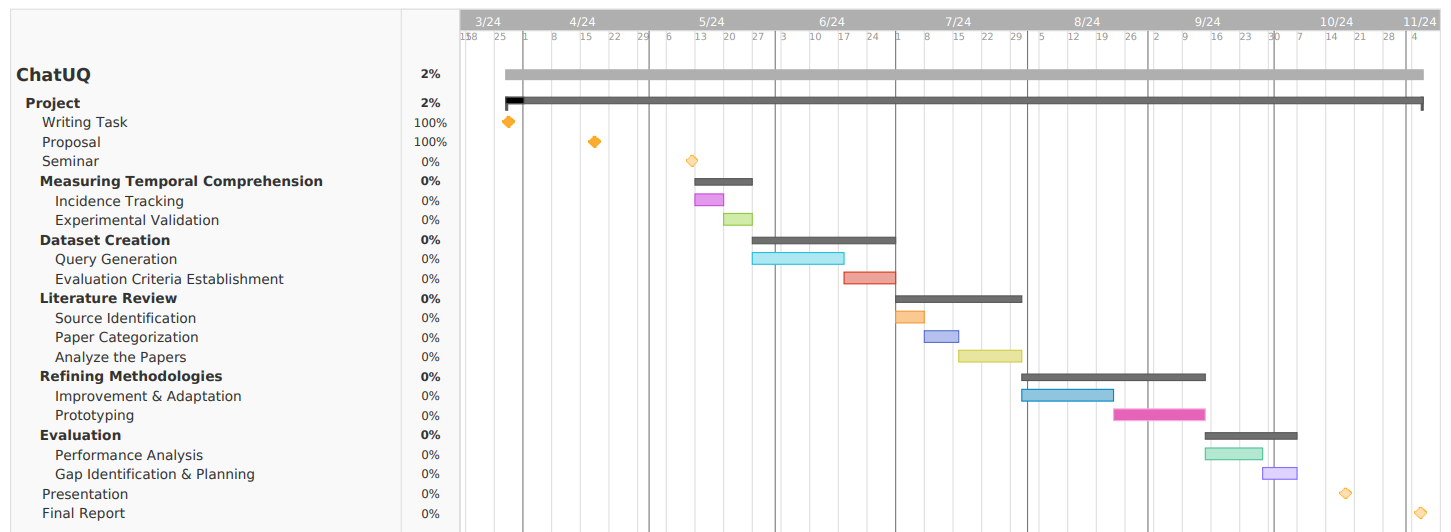
\includegraphics[width=\textwidth]{Gantt Chart.png} \\

Figure 3 is a Gantt Chart representing how each milestone and its subtasks will be achieved. Please note that some activities may be carried out in parallel and dependencies exist, that is, most subtasks/milestones are dependent on the completion of other subtasks/milestones. 

\subsection{Risk Assessment}

\begin{itemize}

\item The experiments that will be needed to be run in this project could be computationally expensive and I might not have enough computational power.

Mitigation: Initial experiments will be scaled down to run only necessary tests and conserve resources. If further computational resources would be needed they would be requested to the EECS school or a budget for cloud computing would be agreed upon with the research group.

\item This project would require dealing with a lot of files including research papers, codes, notes etc., so there could be a risk of loss of files.

Mitigation: Every file related to the project would be pushed to a GitHub repository. Regular checks would be done to assure copies of all files have been uploaded on the GitHub repository.

\item As this project will be moving forward, there is a risk that the research could become outdated when the project is completed.

Mitigation: Regular literature reviews will be conducted to ensure that new technology/research methods are incorporated in my own project. This will help maintain the project's relevance and effectiveness.

\end{itemize}

\subsection{Ethics Assessment}

For this project, I will be exclusively utilizing publicly available data sourced from open datasets. No private or personally identifiable data from users will be involved in any phase of the research. Hence, there is no need to go over the traditional ethical assessment.